\documentclass[elementsmain.tex]{subfiles}
\begin{document}
\section{The Space $\mathbb{R}^m$: Points, Vectors, and Vectors}


Our goal here is to introduce the fundamental object of linear algebra, the vector. The word has slightly different meanings depending on context, so we will to sort this out carefully first in two dimensions, where we can draw the best pictures. Then we will extend the ideas to the general situation.

\subsection*{The Idea of a Vector}

Let's recall the idea of \emph{the plane} from classical geometry: the plane is like a flat sheet of drawing paper, which extends indefinitely in all directions without bound.


You have likely seen the idea of \emph{Cartesian coordinates} on the plane before. To be clear, let's set things down carefully. In the plane, we choose a pair of perpendicular lines which meet at a point $O$. This special point is called the \emph{origin}. Then, we choose a point $X$ on one of the lines and draw the circle centered at $O$ which passes through $X$. Note that this circle meets our two lines in two points each, four points total, one of which is the point $X$. Then we rotate from $X$ around the circle by a quarter turn counterclockwise until we hit one of the points on the other line. We call this new point $Y$. Are you drawing with me? Here is my picture so far.

\begin{figure}[h!]
\centering
\begin{tikzpicture}[scale=2]
\draw (-1,4/3) -- (1,-4/3);
\draw (-3/2,-9/8) -- (3/2,9/8);
\draw (0,0) circle [radius=3/4];
\draw[->] (-50:1) arc (-50:35:1);
\node [right] at (1.1,0) {rotate counterclockwise};
\node [left] at (0,0) {$O$};
\node [below] at (9/20,-13/20) {$X$};
\node [above] at (3/5,9/20) {$Y$};
\end{tikzpicture}
\end{figure}

We call the line $OX$ the \emph{$x$-axis} and the line containing $Y$ the \emph{$y$-axis}. Here comes the amazing part: we declare the circle we used to be of \emph{unit size}, and make the lines $OX$ and $OY$ into number lines! The important part is that the point $O$ should represent $0$ on both number lines, and the points $X$ and $Y$ should each represent $1$ on their lines. So, instead of marking things with $O$, $X$, and $Y$, we put down marks where $X$ and $Y$ are and label them with $1$'s, and add little arrows marked with $x$ and $y$ near the positive ``ends'' of the lines $OX$ and $OY$, respectively.

\begin{figure}[h!]
\centering
\begin{tikzpicture}[scale=1.2]
\draw[->] (-1,4/3) -- (1,-4/3);
\draw[->] (-3/2,-9/8) -- (3/2,9/8);
\draw[fill] (9/20,-3/5) circle [radius=0.03];
\draw[fill] (3/5,9/20) circle [radius=0.03];
\node [below] at (9/20,-3/5) {$1$};
\node [above] at (3/5,9/20) {$1$};
\node [right] at (1,-4/3) {\small $x$};
\node [left] at (3/2,9/8) {\small $y$};
\end{tikzpicture}
\end{figure}

Note that above I have done something a bit silly and let the picture just fall on the paper in an unusual way.
I really mean unusual as ``not usual.''
The usual way arranges the lines on the paper to match our expected horizontal ($x$) and vertical ($y$) directions.
This isn't actually required, but it is what everyone always does.
The typical picture looks like Figure \ref{fig:cartesian-coords}.


\begin{figure}[h]
\centering
\begin{tikzpicture}[scale=1]
\draw[->] (-2,0) -- (2,0) node[below] {\small $x$};
\draw[->] (0,-2) -- (0,2) node[left] {\small $y$};
\draw[fill] (1,0) circle [radius=0.03] node[below] {$1$};
\draw[fill] (0,1) circle [radius=0.03] node[left] {$1$};
\end{tikzpicture}
\caption{The Standard Cartesian Coordinate System}
\label{fig:cartesian-coords}
\end{figure}


Now suppose we have some point in the plane, let's call it $P$.
We can describe the location of $P$ relative to our two lines in a simple way. First, we draw a line through $P$ which is parallel to the $y$-axis and perpendicular to the $x$-axis.
The foot of this perpendicular hits the $x$-axis at some point $A$.
But this point $A$ is part of the number line $OX$, so it has an associated real number, which we will call $a$.
So the point $A$ is instead marked with the label $a$ from this number line.

Similarly, we draw a line through $P$ parallel to the $x$-axis and perpendicular to the $y$-axis.
The foot of this perpendicular hits the $y$-axis at some point $B$, which is part of the number line $OY$.
We denote the number associated to $B$ by $b$.
Again, the point is labeled with the number $b$ from the number line.

\begin{figure}[h!]
\centering
\begin{tikzpicture}[scale=1.2]
\draw[->] (-2,0) -- (2,0) node[below] {\small $x$};
\draw[->] (0,-2) -- (0,2) node[left] {\small $y$};
\draw[fill] (-1/2,3/4) circle [radius=0.03] node[below left] {$P$};
\draw[dotted] (-1/2,-2) -- (-1/2,2);
\draw[dotted] (-2,3/4) -- (2,3/4);
\draw (-.05,3/4) -- (.05,3/4) node[above right] {$b$};
\draw (-1/2,.05) -- (-1/2,-.05) node[below left] {$a$};
\end{tikzpicture}
\caption{A point $P$ and its coordinates $(a,b)$.}
\label{fig:point-coords}
\end{figure}

So, to identify the point $P$, we can instead give the pair of numbers $a$ and $b$.
These numbers are called the \emph{coordinates} of $P$.
Of course, the order of the coordinates matters, so we make what we call an \emph{ordered pair} $(a,b)$ to keep things straight, where the $x$-coordinate comes first, and the $y$-coordinate comes second. Note that in Figure \ref{fig:point-coords} the $x$-coordinate $a$ is negative, but the $y$-coordinate $b$ is postive.

This whole process is reversible, too. If we pick a pair of numbers $c$ and $d$, in order, then we can find a point in the plane which corresponds, and we can do it unambiguously. Find the spot labeled $c$ on the $x$-axis number line and construct a line perpendicular to the $x$-axis through this point. Similarly, find the spot labeled $d$ on the $y$-axis and construct a line perpendicular to the $y$-axis through this point. The two lines you just drew will meet in exactly one point $Q$, and $Q$ will have coordinates $(c,d)$.

This setup of coordinates on the plane allows us to formalize a wonderful and useful idea from physics, too.
Physicists use the concept of a \emph{vector} to describe something (like the wind) which has both magnitude or size (like how fast the air is moving)  and direction (which way the air is going).
Usually, vectors are drawn as little arrows: the arrow has a direction, and it has a length which represents its magnitude.
It is possible to draw vectors which have the same direction but different lengths, and vice versa.

We can use coordinates to describe vectors in the plane, too.
Here's how: A physicist's vector $v$ is some arrow in the plane.
That arrow has an initial point $P$, called its \emph{tail}, and a final point $Q$, called its \emph{head}.
We can write the coordinates of these points as $P = (a,b)$ and $Q = (c,d)$.

\begin{figure}[h]
\centering
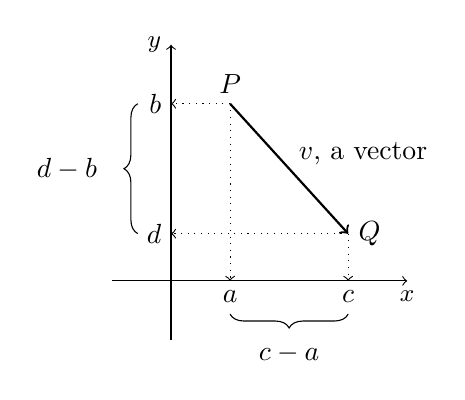
\begin{tikzpicture}[scale=1.5]
\draw[->] (-.5,0) -- (2,0) node[below] {\small $x$};
\draw[->] (0,-.5) -- (0,2) node[left] {\small $y$};
\draw[->,thick] (1/2,3/2) node[above] {$P$} -- (3/2,2/5) node[right] {$Q$};
\node [above right] at (1,18/20) {$v$, a vector};
\draw[dotted,->] (1/2,3/2) -- (1/2,0) node[below] {$a$};
\draw[dotted,->] (1/2,3/2) -- (0,3/2) node[left] {$b$};
\draw[dotted,->] (3/2,2/5) -- (3/2,0) node[below] {$c$};
\draw[dotted,->] (3/2,2/5) -- (0,2/5) node[left] {$d$};
\draw[decorate,decoration={brace,amplitude=5pt},xshift=-8pt,yshift=0pt] (0,2/5) -- (0,3/2) node[midway,xshift=-.9cm] {$d-b$};
\draw[decorate,decoration={brace,mirror,amplitude=5pt},xshift=0pt,yshift=-8pt] (1/2,0) -- (3/2,0) node[midway,yshift=-.5cm] {$c-a$};
\end{tikzpicture}
\caption{Coordinates for a physicist's vector $v$.}
\label{fig:phys-vec-coords}
\end{figure}


Then the coordinates of $v$ are taken to be the numbers $c-a$ and  $d-b$, which we interpret how much $v$ acts in the directions parallel to the $x$-axis and the $y$-axis, respectively.
Note that in Figure \ref{fig:phys-vec-coords}, the $y$-coordinate is negative, since $b>d$.

These coordinates have a hint of algebraic manipulation in them.
Those subtractions line up almost like we could write $v =(c-a,d-b) = (c,d)-(a,b) = Q-P$.
But $v$ is a vector, and if we write it like $(c-a,d-b)$, it looks like the notation for a point.
We should not do that because it could get confusing.
Furthermore, that ``equation'' would mean that we are subtracting points and creating a vector, which is also weird.
Still, there is something to it.
We will return to this idea soon.

For now, let's focus on a bit of ambiguity in the physicist's idea of a vector.
Where should that vector be?
That is, given the coordinates of a vector in the plane, it is not clear where to draw it!
We can slide a vector around the plane, and as long as we keep it parallel to the original, the coordinates won't change.
So, unlike the coordinates of a point, the coordinates of a vector do not uniquely specify the vector.

The mathematician's special fix is this: we simply declare all our vectors to have their initial points, their tails, at the point $O$, the origin of our coordinate system.
That curtails some of the (admittedly useful) freedom in the physics notion, but it also lets us be more clear.

\begin{figure}[h]
\centering
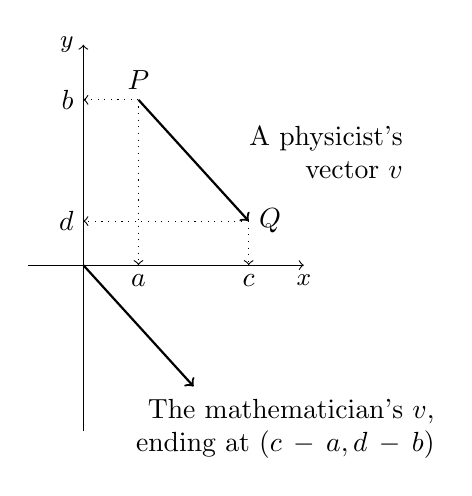
\begin{tikzpicture}[scale=1.4]
\draw[->] (-.5,0) -- (2,0) node[below] {\small $x$};
\draw[->] (0,-1.5) -- (0,2) node[left] {\small $y$};
\draw[->,thick] (1/2,3/2) node[above] {$P$} -- (3/2,2/5) node[right] {$Q$};
\node [text width=3cm,align=right,above right] at (2/3,14/20) {A physicist's\\ vector $v$};
\draw[dotted,->] (1/2,3/2) -- (1/2,0) node[below] {$a$};
\draw[dotted,->] (1/2,3/2) -- (0,3/2) node[left] {$b$};
\draw[dotted,->] (3/2,2/5) -- (3/2,0) node[below] {$c$};
\draw[dotted,->] (3/2,2/5) -- (0,2/5) node[left] {$d$};
\draw[->,thick] (0,0) -- (1,-11/10);
\node [text width=5cm,align=right,below] at (7/5,-9/8) {The mathematician's $v$,\\ ending at $(c-a,d-b)$};
\end{tikzpicture}
\caption{The physicist's vector vs. the mathematician's vector.}
\end{figure}

It pays to keep in mind that the physicists conception of the vector $V$ with coordinates $c-a$ and $d-b$ could be one of many different arrows, while the mathematician's vector $v$ is the arrow from the point $O = (0,0)$ to the point $(c-a, d-b)$.

Now we have circled back around to a muddle. If a mathematician's vector is always based at $O$, we only need to specify where the head of the vector is\dots which is just a point. So, how is a vector supposed to be different from a point, again?

This confusion of three different, shifting, partially-overlapping interpretations causes some trouble to the new learner.
Professionals tend to pass back and forth between these and use them flexibly to get results.
Once you have gotten used to the ideas, you will, too.
You should watch out for these instances where the words point and vector get interchanged.
If they cause you trouble, remember that we have three different things, which are closely related.

For now, the simplest way to handle things is like this:
\begin{itemize}
\item Ignore the physicist's version of the word vector as much as possible.
\item A point is a location in the plane, and represented by coordinates in the form of an ordered pair of numbers $(a,b)$.
\item A vector is an arrow based at the origin, which can be specified by the coordinates of its head. To keep this separate from the idea of a point, we will write it differently, with the numbers stacked vertically like this: $\smvec{a}{b}$.
\item Always remember that for each point in the plane, there is a unique mathematician's vector which corresponds, and vice versa.
\end{itemize}
With this in mind, we make our first official definition.

\begin{definition} A $2$-vector is a vertical stack of $2$ real numbers, like so:
\[
v = \begin{pmatrix} a \\ b \end{pmatrix}.
\]
The collection of all such $2$-vectors is called \emph{the plane}, and written with this notation: $\R^2$.
\end{definition}

The notation $\R^2$ is often read ``arr-two,'' and many people use that language interchangeably with ``the plane.'' Also, most of the time we will just say ``vector,'' rather than ``$2$-vector.'' 

\subsection*{Vector Algebra}

Let's return to that glimpse of subtraction we saw in Figure \ref{fig:phys-vec-coords}.
We saw there that for points $P = (a,b)$ and $Q = (c,d)$, the vector $v$ from $P$ to $Q$ has coordinates $c-a$ and $d-b$.
This looks almost like we subtracted the points to get $Q-P = v$.
Can we use that?
The weird part is that it mixes up points and vectors.
So, we change viewpoints, and instead think of $P$ and $Q$ as (mathematician's) vectors. To keep things clear, let's introduce new labels.
\[
p = \begin{pmatrix} a \\ b \end{pmatrix}, \quad q = \begin{pmatrix} c \\ d \end{pmatrix}
\]
If we put these together on the plane with the physicist's vector $v$ from $p$ to $q$ and the mathematician's $v$ we see a wonderful triangle, and an extra vector.
\begin{figure}[h]
\centering
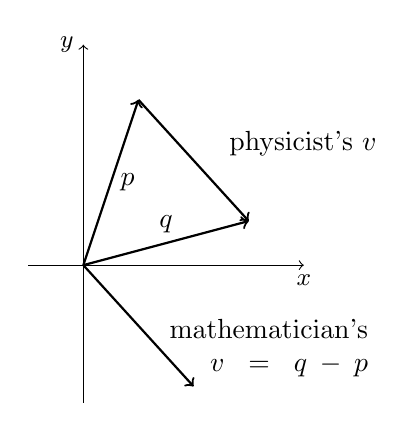
\begin{tikzpicture}[scale=1.4]
\draw[->] (-.5,0) -- (2,0) node[below] {\small $x$};
\draw[->] (0,-1.25) -- (0,2) node[left] {\small $y$};
\draw[->,thick] (1/2,3/2) -- (3/2,2/5);
\node [text width=2.2cm,align=right,above right] at (1,18/20) {physicist's $v$};
\draw[->,thick] (0,0) -- (1,-11/10);
\node [text width=3.5cm,align=right] at (4/3,-3/4) {mathematician's $v=q-p$};
\draw[->,thick] (0,0) -- (1/2,3/2);
\node[right] at (1/4,3/4) {$p$};
\draw[->,thick] (0,0) -- (3/2,2/5);
\node[above] at (3/4,1/5) {$q$};
\end{tikzpicture}
\caption{Subtraction of vectors}
\label{fig:subtract-vec}
\end{figure}
So we see a way to talk about subtracting vectors: Given two vectors $p$ and $q$ as above, their
\emph{difference} is the vector
\[
V = Q-P = \begin{pmatrix} c \\ d \end{pmatrix} - \begin{pmatrix} a \\ b \end{pmatrix} = \begin{pmatrix} c-a \\ d-b \end{pmatrix}.
\]
Geometrically, we draw the arrow from $p$ to $q$ and then translate it down so that its tail is at the origin $O=(0,0)$. Of course, the order of $p$ and $q$ in this operation matters. If we switch them, we get an arrow pointing in the opposite direction.

If we can subtract vectors, surely we can add vectors. How would that work? Algebraically, if $v=q-p$, then we expect $q=v+p$ by rearranging.
That would mean
\[
q = \begin{pmatrix} c \\ d \end{pmatrix} = v+p = \begin{pmatrix} c-a \\ d-b \end{pmatrix} + \begin{pmatrix} a \\ b \end{pmatrix},
\]
which all fits. It looks like addition should be defined coordinate-by-coordinate.

\begin{definition}[Addition of Vectors]
Let $p = \smvec{a}{b}$ and $q= \smvec{c}{d}$ be two vectors in $\R^2$. Their sum is the vector
\[
p+q = \begin{pmatrix} a+c \\ b+d\end{pmatrix}.
\]
\end{definition}

\begin{theorem}\label{thm:vect-add}
Addition of vectors satisfies the same rules as addition of real numbers:
\begin{compactitem}
\item when adding more than two vectors, it doesn't matter which operations you do first:
$(p+q)+r = p + (q+r)$;
\item one can add in either order $p+q = q+p$;
\item the vector $0$ corresponding to the origin $O$ is a ``zero'' since $p+0 = 0+p = p$;
\item for each vector $p$, there is an opposite vector $-p$ so that $p + (-p) = 0$.
\end{compactitem}
\end{theorem}

\begin{readingex}
Remember that you are supposed to read actively.
You can draw all of these pictures and try out all of these things with specific examples that you invent.
You should check the statements in Theorem \ref{thm:vect-add} by making examples and working out the details.
Can you also draw the pictures which go with your examples?
\end{readingex}


But what about subtracting geometrically? In Figure \ref{fig:subtract-vec}, I have a strong desire to complete the figure by joining the loose end of $v$ to the rest of the figure. If we draw the arrow from the head of $v$ to the head of $q$, we get Figure \ref{fig:add-vec}.
\begin{figure}[h!]
\centering
\begin{subfigure}[b]{0.45\textwidth}
    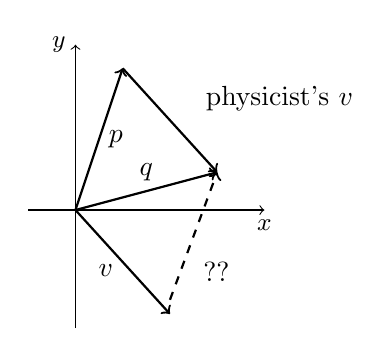
\begin{tikzpicture}[scale=1.2]
    \draw[->] (-.5,0) -- (2,0) node[below] {\small $x$};
    \draw[->] (0,-1.25) -- (0,1.75) node[left] {\small $y$};
    \draw[->,thick] (1/2,3/2) -- (3/2,2/5);
    \node [text width=2.2cm,align=right,above right] at (1,19/20) {physicist's $v$};
    \draw[->,thick] (0,0) -- (1,-11/10);
    \node [below left] at (1/2,-19/40) {$v$};
    \draw[->,thick] (0,0) -- (1/2,3/2);
    \node[right] at (1/4,3/4) {$p$};
    \draw[->,thick] (0,0) -- (3/2,2/5);
    \node[above] at (3/4,1/5) {$q$};
    \draw[->,dashed,thick] (1,-19/20) -- (3/2,2/5);
    \node[right] at (5/4,-13/20) {??};
    \end{tikzpicture}
    \caption{Subtraction of vectors}
    \label{fig:add-vec}
\end{subfigure}
\quad
\begin{subfigure}[b]{0.45\textwidth}
    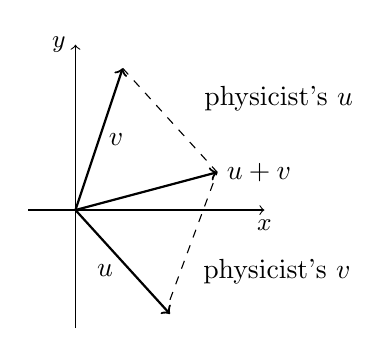
\begin{tikzpicture}[scale=1.2]
    \draw[->] (-.5,0) -- (2,0) node[below] {\small $x$};
    \draw[->] (0,-1.25) -- (0,1.75) node[left] {\small $y$};
    \draw[-,dashed] (1/2,3/2) -- (3/2,2/5);
    \node [text width=2.2cm,align=right,above right] at (1,19/20) {physicist's $u$};
    \draw[->,thick] (0,0) -- (1,-11/10);
    \node [below left] at (1/2,-19/40) {$u$};
    \draw[->,thick] (0,0) -- (1/2,3/2);
    \node[right] at (1/4,3/4) {$v$};
    \draw[->,thick] (0,0) -- (3/2,2/5);
    %\node[above] at (3/4,1/5) {$A+B$};
    \draw[-,dashed] (1,-19/20) -- (3/2,2/5) node[right] {$u+v$};
    \node[right] at (5/4,-13/20) {physicist's $v$};
    \end{tikzpicture}
    \caption{Geometric Addition of Vectors}
    \label{fig:geom-add-vec}
\end{subfigure}
\caption{Some algebra of vectors}
\end{figure}

What should the label on the dashed vector in Figure \ref{fig:add-vec} be? Just as the physicist's $v$ and the
mathematician's $v$ are parallel, this new vector is parallel to the mathematician's vector $p$.
So the dashed vector must be a physicist's version of $p$. Then we see $q=v+p$.

Now we know how to add geometrically: to add two vectors $u$ and $v$, translate $v$ until its tail is on the head of $u$, then draw a new vector $u+v$ as the vector from the tail of $u$ to the head of this translated $v$. It just repurposes the structure of Figure \ref{fig:add-vec}. This is called the \emph{parallelogram rule} for addition of vectors.

There is another useful operation on vectors called \emph{scalar multiplication}.
The terminology comes from physics (again) where a \emph{scalar} quantity is just a number, and not a vector.
So ``scalar multiplication'' means to multiply a vector by a scalar.


\begin{definition}[Scalar Multiplication for vectors]
Let $p = \smvec{a}{b}$ be a vector in $\R^2$, and let $\lambda$ be a real number. Then the \emph{scalar multiple} $\lambda p$ is defined to be
\[
\lambda p = \begin{pmatrix} \lambda a \\ \lambda b \end{pmatrix}
\]
\end{definition}

If you have never seen the symbol $\lambda$ before, it is an old Greek letter pronounced ``lamb-duh.'' It is traditional to use it in linear algebra in lots of places. Welcome to the $\lambda$-club. Oh, there are other such letters, like $\mu$, which is pronounced ``myoo.''

Again, this operation has some important similarities to the familiar multiplication of numbers, but because it combines a scalar (a number) with a vector (not a number, exactly) to produce another vector (again, not a number) things are a little different.

\begin{theorem}\label{thm:scalar-mult}
Suppose that $p$ and $q$ are vectors, and $\lambda$ and $\mu$ are numbers. Scalar multiplication has the following properties:
\begin{compactitem}
\item Scalar multiplication distributes over vector addition:\\ $\lambda(p+q) = \lambda p + \lambda q$;
\item Scalar multiplication distributes over scalar addition:\\ $(\lambda + \mu)p = \lambda p + \mu q$;
\item Scalar multiplication and regular multiplication can be done in either order: $\lambda(\mu p) = (\lambda\mu) p$;
\item if $\lambda = 0$, then $\lambda p = 0 p = 0$ is the zero vector.
\item if $n$ is a counting number, then $np$ is the same thing as adding together $n$ copies of $p$. In particular, $1p = p$.
\end{compactitem}
\end{theorem}

This Theorem, like the last one, says that some natural properties you hope will still work really do still work. When you study \textbf{Modern Algebra}, making lists of these kinds of properties will be really useful. So far, we have collected up the properties that describe a \emph{vector space}.


What is the geometry of scalar multiplication?
It corresponds to stretching (or shrinking) a vector, without changing its direction.
Let $\lambda$ be a non-zero number. Since
\[
\lambda p = \lambda \begin{pmatrix} a \\ b \end{pmatrix} = \begin{pmatrix} \lambda a \\ \lambda b\end{pmatrix},
\]
we see that the ratio of the two coordinates of a vector doesn't change under scalar multiplication. This means that $p$ and $\lambda p$ point in the same direction.
One can see this by considering similar triangles with sides parallel to the $x$-axis, the $y$-axis, and $p$.

\begin{figure}[h!]
\centering
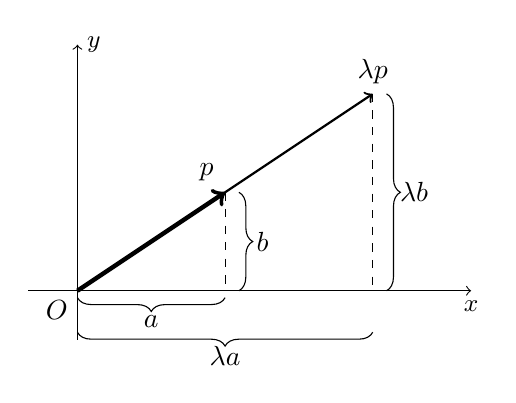
\begin{tikzpicture}[scale=1.25]
\draw[->] (-.5,0) -- (4,0) node[below] {\small $x$};
\draw[->] (0,-.5) -- (0,2.5) node[right] {\small $y$};
\node[below left] at (0,0) {$O$};
\draw[->,thick] (0,0) -- (3,2) node[above] {$\lambda p$};
\draw[->,ultra thick] (0,0) -- (1.5,1) node[above left] {$p$};
\draw[dashed] (1.5,1) -- (1.5,0);
\draw[dashed] (3,2) -- (3,0);
\draw[decorate,decoration={brace,mirror,amplitude=5pt},xshift=4pt,yshift=0pt] (3,0) -- (3,2) node[midway,xshift=.35cm] {$\lambda b$};
\draw[decorate,decoration={brace,mirror,amplitude=5pt},xshift=4pt,yshift=0pt] (1.5,0) -- (1.5,1) node[midway,xshift=.3cm] {$b$};
\draw[decorate,decoration={brace,mirror,amplitude=5pt},xshift=0pt,yshift=-2pt] (0,0) -- (1.5,0) node[midway,yshift=-.3cm] {$a$};
\draw[decorate,decoration={brace,mirror,amplitude=5pt},xshift=0pt,yshift=-12pt] (0,0) -- (3,0) node[midway,yshift=-.3cm] {$\lambda a$};
\end{tikzpicture}
\caption{Similar triangles and scalar multiplication, $\lambda >1$}
\label{fig:sim-tri}
\end{figure}

The triangles in Figure \ref{fig:sim-tri} are similar: their corresponding horizontal and vertical sides are parallel, and those pairs of sides have a common ratio.
We learn that $p$ and $\lambda p$ lie in the same line.

This is important! Later we will describe lines in the plane, and we have just discovered how scalar multiplication relates to those lines which pass through the origin, $O$.

By the way, this picture helps explain the terminology. The vector $\lambda p$ is a rescaled version of $p$. A \emph{scalar} is a thing which \emph{scales} vectors.

\subsection*{The General Case}

Now we can give the fully general definition.

\begin{definition}
Let $m$ be a counting number. We define an $m$-vector to be a vertical stack of $m$ real numbers, like so:
\[
u = \begin{pmatrix} u_1 \\ u_2 \\ \vdots \\ u_m \end{pmatrix} .
\]
The individual entries $u_i$ of $u$ are called its \emph{components}.
The collection of all $m$-vectors is called \emph{$m$-space}, and denoted $\mathbb{R}^m$.
\end{definition}

The symbol $\R^m$ is usually read as ``arr-em.''


\begin{definition}[Linear Combinations of vectors]
Suppose that $u$ and $v$ are two $m$-vectors. Their \emph{sum} $u+v$ is defined by adding the individual components in corresponding positions. If $\lambda$ is a number, then the \emph{scalar multiple} $\lambda u$ is defined by multiplying each of the components of $u$ by the number $\lambda$.

Suppose that $v_1$, $v_2$, \dots, $v_k$ are all $m$-vectors, and that $a_1$, $a_2$, \dots, $a_k$ are all real numbers. Then the vector 
\[
a_1 v_1 + a_2 v_2 + \dots + a_k v_k
\]
is called a \emph{linear combination of the vectors $v_1$, $v_2$, \dots, $v_k$ with weights  $a_1$, $a_2$, \dots, $a_k$}.
\end{definition}

It is much harder to think through the geometry of $\R^m$ when $m$ is large, but the algebra works in much the same way.

\begin{theorem} Fix a natural number $m$. The results of Theorem \ref{thm:vect-add} and Theorem \ref{thm:scalar-mult} about the algebra of vectors hold for vectors in $\R^m$, too.
\end{theorem}

Now that we have a little bit of algebraic structure for vectors, we can form equations.

\begin{definition}
An equation of the form $\lambda_1 u_1 + \dots \lambda_n u_n = w$, where all of the vectors $u_i$ and $w$ are known, but the scalars $\lambda_i$ are unknown, is called a \emph{linear combination of vectors equation}.
A \emph{solution} to such an equation is 
a collection of scalars which make the equation true.
\end{definition}




\clearpage

\subsection*{Exercises}

\begin{exercise}
Write down three distinct points in the plane in proper notation. 
Plot those three points on a single diagram.
\end{exercise}

\begin{exercise}
Write down three distinct vectors in the plane in proper notation. 
Your three points from this task should NOT match any of the three points from the previous task.
Plot those three vectors on a single diagram.
\end{exercise}



\begin{exercise}
Find the sum of your three vectors from the last exercise. Then, choose some order of those three vectors so that they are $u_1$, $u_2$ and $u_3$, and compute the linear combination
\[
3u_1 - 2u_2 + (1/2)u_3.
\] 
\end{exercise}

\begin{exercise}
Let's consider the vectors $u=\left(\begin{smallmatrix} 2 \\1 \end{smallmatrix}\right)$, 
$v=\left(\begin{smallmatrix} 1\\ 1 \end{smallmatrix}\right)$, and $w=\left(\begin{smallmatrix} -3\\ 1 \end{smallmatrix}\right)$.
Compute all of the vectors in this list:
\[
\dfrac{u+v}{2}, v-u, v-w, u + \left(\dfrac{v-u}{3}\right), u + \left(\dfrac{3(v-u)}{4}\right)
\]
Then make a single diagram which contains $u$, $v$, $w$ and all of those vectors from the list, plotted as accurately as you can.

What do you notice? Is anything interesting going on?
\end{exercise}

\begin{exercise}
Consider the vector $u = \left(\begin{smallmatrix} -4 \\ 2\end{smallmatrix}\right)$. Find a vector $v$ which has the property that $u+v$ is the zero vector, or explain why this is not possible.
\end{exercise}


\begin{exercise}
For now, keep $u = \left(\begin{smallmatrix} -4 \\ 2\end{smallmatrix}\right)$. 
Let $v = \left(\begin{smallmatrix} 3 \\ 5 \end{smallmatrix}\right)$.
How many solutions does the linear combination of vectors equation
$\lambda u = v$
have?

How many solutions does the linear combination of vectors equation 
$\lambda u + \mu v = 0$
have? (Here, treat $0$ as the zero vector.)
\end{exercise}

\begin{exercise}
We still use the notation $u$ for the vector $u = \left(\begin{smallmatrix} -4 \\ 2\end{smallmatrix}\right)$, but now use $v$ for the vector $v = \left(\begin{smallmatrix} 28 \\ -14\end{smallmatrix}\right)$.
How many solutions does the linear combination of vectors equation $\lambda u = v$
have?

How many solutions does the linear combination of vectors equation 
$\lambda u + \mu v = 0$ have? (Again, treat $0$ as the zero vector.)
\end{exercise}

\begin{exercise}
Find the midpoint between the points $P = (4,-2)$ and $Q=(3,5)$. Then find the two points which divide the segment $PQ$ into thirds.

How can vectors make this simpler than it first appears?
\end{exercise}

\begin{challenge}
Suppose you are given three points in the plane. Let's call them $P$, $Q$, and $R$.
How can you use vectors to (quickly) determine if these three points are collinear?
\end{challenge}

\begin{exercise}
Write down four $3$-vectors of your choosing, where none has any coordinate equal to $0$. Call these vectors $u_1$, $u_2$, $u_3$, and $u_4$. Now choose any four non-zero scalars you like, call them $\lambda_1$, $\lambda_2$, $\lambda_3$ and $\lambda_4$. Compute the linear combination
\[
\lambda_1 u_1 + \lambda_2 u_2 + \lambda_3 u_3 + \lambda_4 u_4. 
\]
\end{exercise}



\clearpage
\end{document}